\documentclass[11pt]{article}
\usepackage[margin=1in]{geometry}
\usepackage{graphicx}
\usepackage{booktabs}
\usepackage{float}
\usepackage{hyperref}
\usepackage{url}
\usepackage[normalem]{ulem}
\usepackage{listings}
\usepackage{xcolor}

\lstdefinestyle{ccode}{
    language=C,
    basicstyle=\ttfamily\footnotesize,
    keywordstyle=\color{blue},
    commentstyle=\color{gray!70!black}\itshape,
    stringstyle=\color{orange!80!black},
    numbers=left,
    numberstyle=\tiny\color{gray},
    numbersep=8pt,
    breaklines=true,
    showstringspaces=false,
    tabsize=2,
}
\lstset{style=ccode}

\title{Benchmark Results}
\author{}
\date{}

\begin{document}
\maketitle
\tableofcontents
\newpage

\section{ML2 benchmark}
ML2: L2 resident (depending on LFSR settings) linked list traversal

\subsection{Greedy}

\begin{figure}[H]
\centering
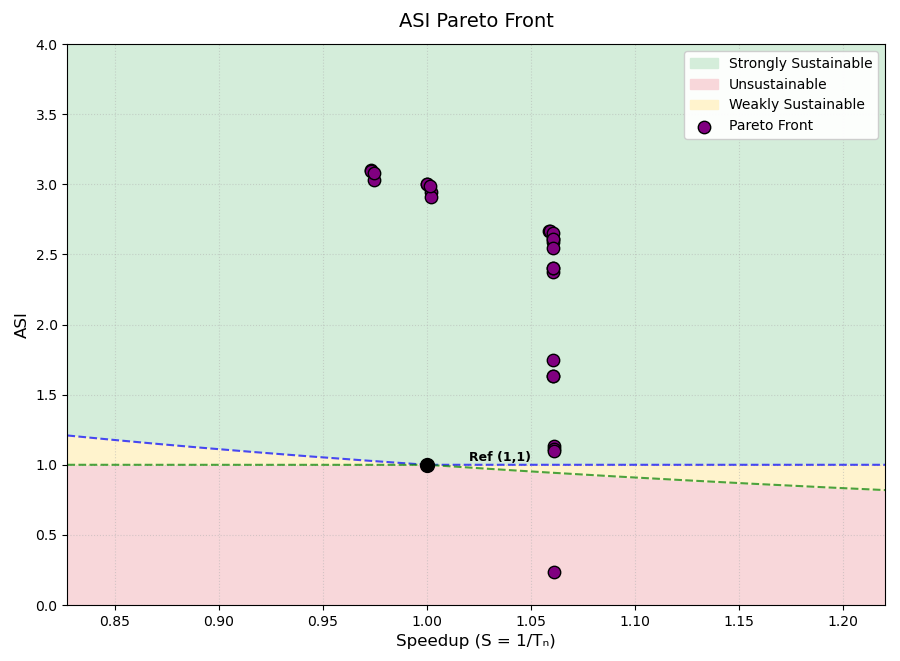
\includegraphics[width=0.48\textwidth]{../../images_results/ML2_greedy.png}
\end{figure}

\textbf{Result:}
\newline
Total sniper runs: 781
\newline
Final hypervolume: 3.2594

\textbf{Front:}

\begin{table}[H]
\centering
\resizebox{\textwidth}{!}{%
\begin{tabular}{lllllllllllllllllll}
\toprule
bpt & bp & l1da & l1d & l1ia & l1i & l2a & l2 & l3a & l3 & nhist & robc & robd & robw & ASI & Speedup & Area & PeakPow & Region \\
\midrule
a53 &  & 4 & 64 &  &  &  & 512 &  & 2048 & 4 &  &  & 1024 & 0.2323 & 1.0610 & 67.94 & 141.87 & Unsustainable \\
pentium\_m &  & 4 & 64 & 8 & 16 &  & 512 &  & 1024 &  & 8 & 2 & 1024 & 1.1008 & 1.0610 & 49.33 & 34.59 & Strongly Sust. \\
pentium\_m &  & 4 & 64 & 8 &  &  & 512 & 4 & 1024 &  & 2 & 2 & 1024 & 1.1154 & 1.0609 & 47.61 & 34.56 & Strongly Sust. \\
pentium\_m &  & 4 & 64 &  &  &  & 512 &  & 1024 &  &  & 2 & 1024 & 1.1342 & 1.0608 & 47.96 & 33.90 & Strongly Sust. \\
a53 &  &  & 64 &  &  &  & 512 &  & 2048 &  & 2 &  &  & 1.6355 & 1.0608 & 55.79 & 22.20 & Strongly Sust. \\
a53 & 512 &  & 64 &  &  &  & 512 &  & 2048 &  & 2 &  &  & 1.6355 & 1.0608 & 55.79 & 22.20 & Strongly Sust. \\
a53 &  &  & 64 &  &  &  & 512 &  & 2048 &  &  &  & 16 & 1.7450 & 1.0607 & 55.19 & 20.90 & Strongly Sust. \\
a53 & 512 &  & 64 &  &  &  & 512 &  & 1024 &  &  & 2 &  & 2.3749 & 1.0607 & 47.80 & 16.21 & Strongly Sust. \\
pentium\_m &  & 4 & 64 & 8 &  &  & 512 &  & 1024 &  &  & 2 & 64 & 2.4038 & 1.0607 & 45.04 & 16.33 & Strongly Sust. \\
a53 & 512 & 4 & 64 & 8 &  &  & 512 &  & 1024 &  &  & 2 & 64 & 2.4038 & 1.0606 & 45.04 & 16.33 & Strongly Sust. \\
a53 & 512 & 4 & 64 &  &  &  & 512 &  & 1024 &  &  & 2 & 64 & 2.5447 & 1.0606 & 43.32 & 15.61 & Strongly Sust. \\
a53 &  & 4 & 64 &  &  &  & 512 & 8 & 1024 &  &  & 2 & 64 & 2.5897 & 1.0606 & 41.24 & 15.56 & Strongly Sust. \\
a53 & 512 & 4 & 64 &  &  &  & 512 &  & 1024 &  &  & 2 & 16 & 2.6083 & 1.0606 & 43.17 & 15.25 & Strongly Sust. \\
a53 &  & 4 & 64 &  &  &  & 512 &  & 1024 &  &  & 2 & 16 & 2.6083 & 1.0605 & 43.17 & 15.25 & Strongly Sust. \\
a53 &  & 4 & 64 &  &  &  & 512 & 8 & 1024 &  &  & 2 & 16 & 2.6546 & 1.0605 & 41.09 & 15.19 & Strongly Sust. \\
a53 &  & 4 &  &  &  &  & 512 & 8 & 1024 &  &  & 2 & 16 & 2.6666 & 1.0589 & 40.92 & 15.14 & Strongly Sust. \\
a53 &  & 4 &  &  &  &  & 512 & 4 & 1024 &  &  & 2 & 16 & 2.6682 & 1.0589 & 40.92 & 15.13 & Strongly Sust. \\
a53 &  & 4 & 64 &  &  & 4 &  &  & 1024 &  &  & 2 & 32 & 2.9076 & 1.0019 & 36.49 & 14.31 & Strongly Sust. \\
a53 &  & 4 & 64 &  &  & 4 &  &  & 1024 &  &  & 2 & 16 & 2.9477 & 1.0018 & 36.40 & 14.12 & Strongly Sust. \\
a53 &  & 4 & 64 &  &  &  &  & 8 & 1024 &  &  & 2 & 16 & 2.9861 & 1.0013 & 34.86 & 14.08 & Strongly Sust. \\
a53 &  & 4 &  &  &  &  &  & 8 & 1024 &  &  & 2 & 16 & 3.0002 & 0.9999 & 34.69 & 14.03 & Strongly Sust. \\
a53 &  & 4 &  &  &  &  &  & 4 & 1024 &  &  & 2 & 16 & 3.0022 & 0.9999 & 34.69 & 14.02 & Strongly Sust. \\
a53 &  & 4 & 64 &  &  & 4 & 128 &  & 1024 &  &  & 2 & 16 & 3.0325 & 0.9746 & 35.43 & 13.81 & Strongly Sust. \\
a53 &  & 4 & 64 &  &  &  & 128 & 8 & 1024 &  &  & 2 & 16 & 3.0823 & 0.9744 & 33.37 & 13.77 & Strongly Sust. \\
a53 &  & 4 &  &  &  &  & 128 & 8 & 1024 &  &  & 2 & 16 & 3.0970 & 0.9732 & 33.20 & 13.72 & Strongly Sust. \\
a53 &  & 4 &  &  &  &  & 128 & 4 & 1024 &  &  & 2 & 16 & 3.0991 & 0.9731 & 33.20 & 13.71 & Strongly Sust. \\
\bottomrule
\end{tabular}
}
\end{table}

\section{Benchmarks}
\subsection{ML2}
ML2: L2 resident (depending on LFSR settings) linked list traversal.

\begin{lstlisting}[caption={ML2 benchmark source}]
#include <stdio.h>
#include <stdlib.h>     /* malloc, free, rand */

#include "common.h"

#define ASIZE 65536*4
#define STEP    128
#define ITERS  4096
#define LEN    2048


typedef struct dude {
  int p1,p2,p3,p4;
} dude;


dude arr[ASIZE];
__attribute__ ((noinline))
int loop(int zero) {
  int t = 0, count=0;

  unsigned lfsr = 0xACE1u;
  do
  {
      /* taps: 18 17 16 13; feedback polynomial: x^18 + x^17 + x^16 + x^13 + 1 */
      lfsr = (lfsr >> 1) ^ (-(lfsr & 1u) & 0x39000u);
      lfsr = lfsr + arr[lfsr].p1;
  //} while(++count < ITERS);
  } while(lfsr != 0xACE1u);

  return t;
}


int main(int argc, char* argv[]) {
   argc&=10000;
   ROI_BEGIN();
   int t=loop(argc);
   ROI_END();
   volatile int a = t;
}
\end{lstlisting}

\subsection{CCl}
CCl: Impossible control with large basic blocks (potentially larger penalty)

\begin{lstlisting}[caption={CCl benchmark source}]
    #include <stdio.h>
#include "randArr.h"
#include "common.h"

#define ASIZE 2048
#define STEP   256
#define ITERS    8

__attribute__ ((noinline))
int loop(int zero) {
  int t = 0,i,iter;
  for(iter=0; iter < ITERS; ++iter) {
    for(i=0; i < STEP + zero; i+=1) {
      if(randArr[i])  {
        t+=3+3*t;
        t&=0xFFF;
        t+=3+3*t;
        t&=0xFFF;
        t+=3+3*t;
        t&=0xFFF;
        t+=3+3*t;
        t&=0xFFF;
        t+=3+3*t;
        t&=0xFFF;
        t+=3+3*t;
        t&=0xFFF;
        t+=3+3*t;
        t&=0xFFF;
        t+=3+3*t;
        t&=0xFFF;
        t+=3+3*t;
        t&=0xFFF;
      } else {
        t&=0xFFF;
        t+=3+3*t;
        t&=0xFFF;
        t+=3+3*t;
        t&=0xFFF;
        t+=3+3*t;
        t&=0xFFF;
        t+=3+3*t;
        t&=0xFFF;
        t+=3+3*t;
        t&=0xFFF;
        t+=3+3*t;
        t&=0xFFF;
        t+=3+3*t;
        t&=0xFFF;
        t+=3+3*t;
        t&=0xFFF;
        t+=3+3*t;
      }
    }
  }
  return t;
}

int main(int argc, char* argv[]) {
   argc&=10000;
   ROI_BEGIN(); 
   int t=loop(argc); 
   ROI_END();
   volatile int a = t;
}

\end{lstlisting}

\subsection{MIP}
MIP: Large Instruction Region -- Instruction cache Misses

\begin{lstlisting}
    #include <stdio.h>
#include "common.h"

#define ASIZE 2048
#define STEP   128
#define ITERS    4

__attribute__ ((noinline))
int loop(int zero) {
  int t = zero,i,iter;
  for(iter=0; iter < ITERS; ++iter) {
    t += 1;
    t *= 2;
    t -= 1;
    t &= 0xFFF00FFF;
    t ^= 0x14022;
    t %= 0xFFFFFF3;
    t += 6;
    t *= 10;
    t += 1;
    t *= 2;
    t -= 1;
    t &= 0xFFF00FFF;
    t ^= 0x14022;
    t %= 0xFFFFFF3;
    t += 6;
    t *= 10;
    t += 1;
    t *= 2;
    t -= 1;
    t &= 0xFFF00FFF;
    t ^= 0x14022;
    t %= 0xFFFFFF3;
    ...
    t += 1;
    t *= 2;
    t -= 1;
    t &= 0xFFF00FFF;
    t ^= 0x14022;
    t %= 0xFFFFFF3;
    t += 6;
    t *= 10;
  }
  return t;
}

int main(int argc, char* argv[]) {
   argc&=10000;
   ROI_BEGIN(); 
   int t=loop(argc); 
   ROI_END();
   volatile int a = t;
}
\end{lstlisting}

\subsection{EI}
EI:Integer Execution -- 8 Independent computations per iteration 

\begin{lstlisting}
    #include <stdio.h>
#include "common.h"

#define ASIZE 2048
#define STEP   128
#define ITERS 4096

__attribute__ ((noinline))
int loop(int zero) {
  int t1 = 1;
  int t2 = 89;
  int t3 = 3;
  int t4 = 21;
  int t5 = 2;
  int t6 = 7;
  int t7 = 2;
  int t8 = 3;
  int t9 = 1;
  int t10 = 89;
  int t11 = 3;
  int t12 = 21;
  int t13 = 2;
  int t14 = 7;
  int t15 = 2;
  int t16 = 3;

  int i;

  for(i=zero; i < ITERS; i+=1) {
    t1+=i;
    t2+=i;
    t3+=i;
    t4+=i;
    t5+=i;
    t6+=i;
    t7+=i;
    t8+=i;
    t9+=i;
    t10+=i;
    t11+=i;
    t12+=i;
    t13+=i;
    t14+=i;
    t15+=i;
    t16+=i;
  }
  return t1+t2+t3+t4+t5+t6+t7+t8*t9+t10+t11+t12+t13+t14+t15+t16;
}

int main(int argc, char* argv[]) {
   argc&=10000;
   ROI_BEGIN(); 
   int t=loop(argc); 
   ROI_END();
   volatile int a = t;
}

\end{lstlisting}
\end{document}

